\chapter{Evaluation}
To verify our work on the convergence layer as well as compare it to others and
find potential bottlenecks we evaluated our work under different test cases.
Comparing the data throughput and packet loss for raw IEEE 802.15.4 against DTN
as an additional layer was the first test case. This metric allows us to compare
the throughput with other test systems using for example IEEE 802.11.
Furthermore this test case allows us to measure the protocol overhead added by
DTN on top of another connection. The second test case has been Round Trip Time
measurement. It measured the time a packet needs to travel to the destination
and back. Again we gathered a metric we can use to compare against other DTN
test system we have and calculate the delay DTN added to a connection.

All measurements have been repeated for different distances between the nodes.
This way we gathered some implicit informations about the potential range of the
wireless link. Not a real distance measurement but together with a quality
indicator like packet loss an interesting by-product of our other test cases.

\section{Throughput}
For the real payload data throughput we measured the payload data the receiving
nodes could receive over time. We did the measurement for raw IEEE 802.15.4 and
DTN traffic separately. For both test cases we sent packages with the maximum
payload from one node to another as fast as the system allowed. The maximum
payload length for IEEE 802.15.4 packets has been 115 bytes and for DTN 40 bytes.
That means that for our DTN tests we have a ratio of two thirds header to one
third payload. As a consequence this results in lower throughput due to less
actual payload per packet.

During these tests a problem in the lower layers of the system was exposed. It is
still unclear if it is a driver or a problem with the ieee802154 stack. The
problem showed up when we tried to send the packets as fast as possible over the
socket interface. After some packets the kernel part got stuck and stopped
transmitting while still accepting data over the socket. The kernel log output
showed an unbalanced IRQ as a potential reason for this problem. Time did not allow
to go to the ground of this problem and fix it properly so we used a delay
in the test application to circumvent this. We added a 100ms delay in the send
routine and the lookup went away. It was the smallest value we could still
reliable send data with. Obviously such a big delay has a negative impact on the
throughput, but without it no measurement would have been possible at all. Each
measurement was done five times and the values as shown in the graphs are the
arithmetic means of these five values.

Figure~\ref{fig:throughput} shows the data we collected over different distances
between the nodes on the IEEE 802.15.4 layer. While the IEEE 802.15.4 throughput
gradually decreases, the DTN throughput on the left chart of figure~\ref{fig:throughput_dtn}
has some interesting amplitudes and trespasses. They
are related to a problem on the sending node. Every now and then the DTN
communication between our test application and the local DTN daemon would hang
for some seconds and then continue. The hang occurred locally without any bundle
send over the network. Further investigation showed that it must be a problem
with usage of the local API the DTN daemon offers to applications.

While not being able to find the culprit we run another test  cycle and filtered
out all results where a bundle needs more then 5 seconds from the test
application to the DTN daemon. This data is the base for the right graph. Like
the IEEE 802.15.4 graph the throughput decreases over the distance.

Due to the added delay in the testing software the throughput is
not really impressive. The theoretical maximum for IEEE 802.15.4 on the 2.4 GHz
band is about 250 kbps and in our tests we only reached a maximum throughput of
4600 bps which equals 1.8 percent of the theoretical maximum. Channel 11 was used
on the 2.4 GHz band which is the only band our hardware supports.

\begin{figure}
  \begin{center}
    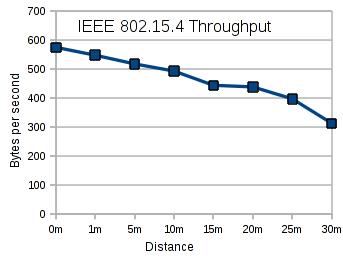
\includegraphics[width=6.5cm]{images/throughput_802154}
    \caption{Data throughput for IEEE 802.15.4}
    \label{fig:throughput}
  \end{center}
\end{figure}

\begin{figure}
  \begin{center}
    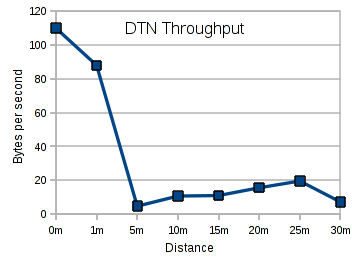
\includegraphics[width=6.5cm]{images/throughput_dtn}
    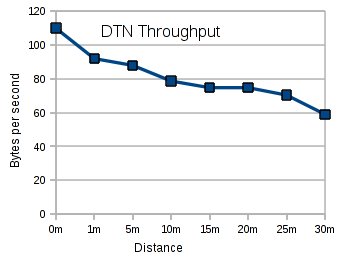
\includegraphics[width=6.5cm]{images/throughput_dtn2}
    \caption{Data throughput for DTN}
    \label{fig:throughput_dtn}
  \end{center}
\end{figure}

\section{Packet loss}
Throughput alone is of course nothing that tells us much about how reliable a
connection is. Therefore we also measured the packet loss while doing the
throughput measurements. Inside the packet payload a sequence number was encoded
and was used to calculate the packet loss rate. No retransmission
was done on the lower layers to avoid even more negative impact on the
throughput and wrong statistics in this test.

Table~\ref{tableloss} shows the constant raise of the lost packet rate over the
distance we did our measurements. On a first look it looked suspicious that the
packet loss for DTN was lower then for IEEE 802.15.4 although DTN was used on top
of IEEE 802.15.4. It can be explained though when keeping in mind that less
packets where sent with DTN in the same time-frame. The latency and short hangs
we already discussed did not allow a higher throughput. The slower sending could
explain the better packet loss rate. The single packet had a smaller probability
to get damaged on the air from other packets and thus have a lower packet loss
rate.

\begin{table}
\begin{tabular}{lllllllll}
    & 0m & 1m & 5m & 10m & 15m & 20m & 25m & 30m \\
\hline
802.15.4 & 0\% & 0\% & 10\% & 10\% & 19\% & 20\% & 31\% & 43\% \\
DTN & 0\% & 0\% & 0\% & 15\% & 15\% & 15\% & 20\% & 30\% \\
\end{tabular}
\caption{Packet loss for IEEE 802.15.4 and DTN over distance}
\label{tableloss}
\end{table}

\section{Distance}
The Imote2 has no connector for an external antenna but an on-board antenna
only. To get an understanding which use cases this antenna, and therefore the
whole board, could cover we combined our measurements with a distance
measurement. To decide if a distance is still usable enough we used the
packet loss as quality indicator. All distances which showed a packet loss above
50 percent are rated as unusable. During our measurements the packet loss
increased over the distance with 43 percent at 30m, as can be seen in table~\ref{tableloss}, and trespassed the 50 percent boarder from 33m upwards.

\begin{table}
\begin{tabular}{lllllllll}
    & 0m & 1m & 5m & 10m & 15m & 20m & 25m & 30m \\
\hline
Min & 656.14 & 651.11 & 664.25 & 645.27 & 659.29 & 651.40 & 653.66 & 677.29 \\
Mean & 676.17 & 662.38 & 674.85 & 674.85 & 676.46 & 672.03 & 672.47 & 686.60 \\
Max & 693.14 & 678.49 & 684.96 & 685.11 & 695.76 & 684.22 & 687.26 & 693.64 \\
\end{tabular}
\caption{DTN Round Trip Time measurement results over IEEE 802.15.4}
\label{dtnrtt}
\end{table}

\begin{table}
\begin{tabular}{lllllllll}
    & 0m & 1m & 5m & 10m & 15m & 20m & 25m & 30m \\
\hline
Min & 442.41 & 437.44 & 440.15 & 437.58 & 436.88 & 437.76 & 438.57 & 437.82 \\
Mean & 442.53 & 438.29 & 441.36 & 437.65 & 437.68 & 438.54 & 441.46 & 440.94 \\
Max & 442.84 & 438.46 & 443.49 & 441.25 & 442.19 & 441.46 & 441.47 & 441.69 \\
\end{tabular}
\caption{IEEE 802.15.4 Round Trip Time measurement results}
\label{802154rtt}
\end{table}
machine.

\section{DTN Round Trip Time}
The last test case was the round trip time of a DTN bundle. We used the
\emph{dtnping} utility to send out a bundle, receive the answer and calculate
the round trip time. Bundles are sent to the \emph{echo} application of the
receiving node. In our case this is directly the DTN daemon. The default payload
size of a ping bundle was too big for our limited payload size on the IEEE
802.15.4 convergence layer. We reduced the payload to 1 byte and used it for all
tests. Table~\ref{dtnrtt} shows the results of the measurement in milliseconds. We
had 10 different scenarios for this test case and did five measurements for each.
The first eight are the same we used for our throughput and packet loss test cases.
In table~\ref{802154rtt} we can see the same measurements without DTN directly on
the IEEE 802.15.4 layer. By comparing these two measurements we can see that DTN
adds a latency around 220ms. More surprising was that IEEE 802.15.4 already had
a latency of about 440ms itself. Even when subtracting the 100ms delay we added
it is still more then expected. We added two more scenarios to compare it against
our usual test environment as can be seen in table~\ref{dtnrtt2}. The
local scenario did send bundles over the UDP convergence layer on the loopback
interface of our x86 workstation while the UDP scenario did send the bundles
through the UDP convergence layer over an 1 Gbit Ethernet link to another

The mean round trip time value does not change much from 0m up to 30m. Actually
the values are so close to each other that they can not be rated relevant. That
is of course no real surprise when the maximum distance is as short as 30m. A
delay for the over the air traveling will not be significant on such a distance.

More interesting is the difference between the round trip time on a IEEE
802.15.4 network in contrast to 1 Gbit Ethernet. With a factor of 16 the latency
added by IEEE 802.15.4 is noticeable. Comparing the value against a
IEEE 802.11 based wireless system could get some insight if this latency is based
on wireless vs. wired or actually on the IEEE 802.15.4 protocol.

\begin{table}
\begin{tabular}{lll}
    & Loopback & Ethernet/UDP \\
\hline
Min & 38.31 & 40.90 \\
Mean & 38.87 & 41.26 \\
Max & 39.41 & 41.56 \\
\end{tabular}
\caption{DTN Round Trip Time measurement results over UDP}
\label{dtnrtt2}
\end{table}
